\documentclass{beamer}
\usepackage{media9}%
\newcommand{\includemovie}[3]{%
\includemedia[%
width=#1,height=#2,%
activate=pagevisible,%
deactivate=pageclose,%
addresource=#3,%
flashvars={%
src=#3 % same path as in addresource!
&autoPlay=true % default: false; if =true, automatically starts playback after activation (see option ‘activation)’
&loop=true % if loop=true, media is played in a loop
&controlBarAutoHideTimeout=0 %  time span before auto-hide
}%
]{}{StrobeMediaPlayback.swf}%
}% end of the new command
\usepackage[utf8]{inputenc}
\usepackage[spanish]{babel}
\usepackage[T1]{fontenc}
\usepackage{booktabs}
\usetheme{JuanLesPins}
\setbeamertemplate{navigation symbols}{}

%Figures Path
\graphicspath{{./imagenes/ResultadosNumericos/RightAngeCantilever/},{./imagenes/ResultadosNumericos/SimpleCable/},{./imagenes/ResultadosNumericos/TransmissionTormenta/}, {./imagenes/Preliminares/Corrotacional/},{./imagenes/Metodologia/},{./imagenes/Anexo/}{./imagenes/Introduccion/}}


%%%%%%%%%%%%%%%%%%%%%%%%%%%%%%%%%%%%%%%%     TITULO  %%%%%%%%%%%%%%%%%%%%%%%%%%%%%%%%%%%%%%%%%
%%%%%%%%%%%%%%%%%%%%%%%%%%%%%%%%%%%%%%%%FRAME%%%%%%%%%%%%%%%%%%%%%%%%%%%%%%%%%%%%%%%%%
\begin{document}

\title[Implementación de una formulación corrotacional en dinámica no lineal y aplicación a líneas de trasmisión]{Implementación de una formulación corrotacional en dinámica no lineal y aplicación al modelado de líneas de transmisión eléctrica }
\author[M.C.\,Vanzulli]{Autor: M.C. Vanzulli$^1$ \\Director de tesis: J.M. Perez Zerpa$^2$ \\ Director de académico: G Usera$^1$ }


\institute [IIMPI-IET]{1-Instituto de Ingeniería Mecánica y Producción Industrial, Facultad de Ingeniería, UdelaR \\ 2-Instituto de Estructuras y Transporte, Facultad de Ingeniería UdelaR  }
\date{\today}
\subject{Presentation Subject}
\keywords{Formulación corrotacional; Método de los Elementos Finitos; Dinámica estructural; Transmisión eléctrica}


%%%%%%%%%%%%%%%%%%%%%%%%%%%%%%%%%%%%%%%%FRAME%%%%%%%%%%%%%%%%%%%%%%%%%%%%%%%%%%%%%%%%%
\begin{frame}[plain]
\maketitle
\end{frame}

\begin{frame}{Table of contents}
\tableofcontents
\end{frame}
%%%%%%%%%%%%%%%%%%%%%%%%%%%%%%%%%%%%%%%%     SECTION  %%%%%%%%%%%%%%%%%%%%%%%%%%%%%%%%%%%%%%%%%
\section[Motivación]{Motivación}

%%%%%%%%%%%%%%%%%%%%%%%%%%%%%%%%%%%%%%%%FRAME%%%%%%%%%%%%%%%%%%%%%%%%%%%%%%%%%%%%%%%%%
\begin{frame}{Motivation}{}


 \begin{block}{¿Por qué? : }
 \begin{itemize}
\item El 10 de marzo de 2002 azotó una tormenta devastadora. Se registraron velocidades de ráfaga de $34$ m/s. Colapsaron:
\begin{itemize}
    \item 19 torres de transmisión eléctrica de $500$ kV.
    \item 48 torres de $150$ kV.
\end{itemize} 
% En el norte de Montevideo los anemómetros capturaron velocidades de ráfaga de $34$ m/s y de acuerdo con el nivel de daño causado, se estimaron que en ciertos puntos podría haber superado los $56$ m/s. Fue tal el nivel de devastación, que 19 torres de transmisión eléctrica de $500$ kV y 48 de $150$ kV colapsaron, además de unos 700 edificios y 1250 techos de hogares que fueron destruidos \citep{duranona2015significance}. Este tornado no solo afectó a las construcciones, sino también muchos productores rurales y sus estancias productivas, derribando invernaderos, montes y plantaciones. El costo de reparación asociado con las torres se estimó en 2 millones de dólares y en simultaneo se destinaron unos 10 millones de dólares a suplir la red con energía geotérmica, proveniente de combustibles fósiles. El presupuesto estimado de los daños en total asciende a la suma de 27 millones de dólares según \cite{duranona2019first}. 
\item  Estudiar el efecto del viento sobre las líneas de alta tensión (500kV) Palmar-Montevideo. Se registraron más de veinte eventos de desconexión en el periodo de 2000-2007.
%Efecto del viento sobre las líneas de alta tensión(500kV) Palmar-Montevideo. Se registraron más de veinte eventos de desconexión en el periodo de 2000-2007.
%más de veinte eventos de desconexión en el periodo de 2000-2007
%Ciertos eventos de vientos severos inducen fuertes movimientos en los cables, provocando un balanceo excesivo de los mismos. Dicho fenómeno puede provocar vulneraciones momentáneas en la aislación del sistema, al aproximar sus cadenas de aisladores a las torres, produciendo descargas a tierra y provocando salidas de servicio temporales de las líneas. (Proyecto VIOLETA ANII)
\end{itemize}
 \end{block}


\begin{figure}[htbp]
	\centering
	\def\svgwidth{80mm}
	\input{./imagenes/Introduccion/Torre.pdf_tex}
	\caption{Ilustración de balanceos excesivos torre Ruta 5.}
	\label{fig:INTRO:IlusExcesiveBalance}
\end{figure}  

 \end{frame}
 
 \begin{frame}
 
\begin{block}{Work's aim (How?):}
\begin{itemize}
\item To illustrate succinctly co-rotational methodology and its principal attractions for modelling structures with large amplitude displacements
%Ilustrar brevemente la metodología corrotacional y sus principales atractivos para el modelado de estructuras con movimientos de gran amplitud.
\item The application of a 3D co-rotational beam element software to high voltage conductors submitted to a downburst storm profile captured experimentally in \cite{Stengel2017a}. 
%Aplicar un software de elementos de viga corrtoacional 3D a conductores de alta tensión ante un perfil de tormenta convectiva capturado experimentalmente en \cite{Stengel2017a}.
 \end{itemize}
 
\end{block}
    \end{frame}

%%%%%%%%%%%%%%%%%%%%%%%%%%%%%%%%%%%%%%%%FRAME%%%%%%%%%%%%%%%%%%%%%%%%%%%%%%%%%%%%%%%%%
%%%%%%%%%%%%%%%%%%%%%%%%%%%%%%%%%%%%%%%%     SECTION  %%%%%%%%%%%%%%%%%%%%%%%%%%%%%%%%%%%%%%%%%
\section[Methodology]{Methodology}
\subsection[Co-rotational formulation]{Co-rotational method}
\subsubsection[Co-rotational kinematics]{Kinematic description of corotational method}

%%%%%%%%%%%%%%%%%%%%%%%%%%%%%%%%%%%%%%%%FRAME%%%%%%%%%%%%%%%%%%%%%%%%%%%%%%%%%%%%%%%%%
\begin{frame}{Co-rotational kinematics}{Reference frameworks}

\begin{figure}[H]
  \centering
    \includegraphics[width=0.33\textwidth]{CinematicaCorrot.jpg}
  \caption{Kinematic description of co-rotational methodology}
 \end{figure}

\begin{itemize}
  \item A global reference system is defined by the orthogonal base $(\bf{e_1},\bf{e_2},\bf{e_3})$
\item Alongside to the element, a framework that moves and rotates solidarity by the triad $(\bf{r_1},\bf{r_2},\bf{r_3})$
 \item To  locate the element on the undeformed and deformed configuration $(\bf{e_1^0},\bf{e_2^0},\bf{e_3^0})$ and $(\bf{t_1^i},\bf{t_2^i},\bf{t_3^i})$ respectively.
   \end{itemize}
\end{frame}



%%%%%%%%%%%%%%%%%%%%%%%%%%%%%%%%%%%%%%%%FRAME%%%%%%%%%%%%%%%%%%%%%%%%%%%%%%%%%%%%%%%%%

\begin{frame}{Co-rotational kinematics}{Global and local coordinates}
\begin{figure}
    \centering
    \def\svgwidth{50mm}
	\input{IlusCorrotacionalDisplacements.pdf_tex}
	\caption{Local and global frameworks.}
    \label{fig:my_label}
\end{figure}

Two types of displacement describing the element are defined:
\pause
\begin{itemize}
\item Global translation and rotation displacements: $\bf{d_g} = (\bf{u_g},\bf{w_g})$
\pause
\item Local linear and angular displacements $\bf{d_l} =(u, \bf{\overline{w_i}}) $
 \end{itemize}

\end{frame}

%\subsubsection[Corotational dynamics]{Dynamic description for internal and dynamics force vector and their respective tangent matrix}

% %%%%%%%%%%%%%%%%%%%%%%%%%%%%%%%%%%%%%%%%FRAME%%%%%%%%%%%%%%%%%%%%%%%%%%%%%%%%%%%%%%%%%


%\begin{frame}{Corotational dynamics}{Internal force vector}

%%   \item Considering the kinematic variables defined previously in combination with the local displacements, the force vectors and the tangent matrices for these coordinates are obtained. Then it is necessary to express them in terms of global displacements. This conversion is calculated by the matrix $\bf{B}$: 
%\begin{center}
%	\begin{equation}
%\bf{\delta d_l}=\bf{B}~\bf{\delta d_g} ~~~~~~ \bf{ f_l}=\bf{B}^T~\bf{ f_g}.
%	\end{equation}
%\end{center}
%\pause
%\item Operating and defining auxiliary variables the internal force vector is obtained: 
% \begin{center}
%	\begin{equation}
%	\bf{F^g_{int}}=\begin{bmatrix} \bf{r}\\ \bf{PE^T} \end{bmatrix} \bf{f_a}
%%	\end{equation}
%\end{center}
%\end{itemize}

%\end{frame}


%%%%%%%%%%%%%%%%%%%%%%%%%%%%%%%%%%%%%%%FRAME%%%%%%%%%%%%%%%%%%%%%%%%%%%%%%%%%%%%%%%%%
%\begin{frame}{Corotational dynamics}{Tangent matrix and inertial force vector}


%\begin{itemize}
 % \item Analogously expressing differential variations of local displacements in global terms, the internal tangent matrix is computed by: 
  %\begin{center}
%	\begin{equation}
%	\bf{K}_{int}^g=\bf{B_a}^T\bf{k_a}\bf{B_a}+\bf{D} f_{a1}-\bf{E}\bf{Q}\bf{G^T}\bf{E^T} +\bf{EGar}
%	\label{eqn:matrizK}
%	\end{equation}
%end{center}
%\pause
%\item The novelty of \cite{Le2014} is based on the consistency of the dynamic terms.This consistency is due to the accurate geometrical characterisation presented previously.  The terms of dynamic forces are responsible for the change of kinetic energy of the element, in turn, by differentiating this, the dynamic tangent matrices are presented;
%\begin{center}
	%\begin{eqnarray}
	%\delta\textit{K}_{din}&=&\bf{f_k^T}\delta\bf{d}^g
	%\label{eqn:defFuerzaInercial} \label{eqn:DefFuerzaInercial}\\
	%\delta\bf{f_k}&=& \bf{M}\delta \ddot{\bf{d_g}}+\bf{C}\delta %\dot{\bf{d_g}}+\bf{K}\delta{\bf{d_g}} \label{eqn:DefMatricesDinamicas}
%	\end{eqnarray}
%\end{center}
%\end{itemize}
%\end{frame}

%%%%%%%%%%%%%%%%%%%%%%%%%%%%%%%%%%%%%%%FRAME%%%%%%%%%%%%%%%%%%%%%%%%%%%%%%%%%%%%%%%%%
%\begin{frame}{Corotational dynamics}{Tangent dynamic matrix}


%\begin{itemize}
%  \item The inertial tangent matrices of Eq. \eqref{eqn:DefMatricesDinamicas} are named:
  
%  \begin{itemize}
%%      \item The consistent mass matrix $\bf{M}$.
 %     \item The gyroscopic matrix $\bf{C}$
 %   \item Finally the centrifugal matrix $\bf{K}$
 % \end{itemize}

%  \pause
  %\item Certain authors such as \cite{cardona1988beam} and \cite{hsiao1999consistent} propose to consider only $\bf{M}$, however exhaustive studies in \cite{hsiao1999consistent} suggest that adding the $\bf{C_k}$ matrix the computational performance is improved.  Now a date, according to the author's knowledge  \cite{Le2014}, any commercial software uses cortoational formulations for the resolution of dynamic problems.
  %\item These matrix could be represented using complex step method. 
   % \end{itemize}
%\end{frame}
%%%%%%%%%%%%%%%%%%%%%%%%%%%%%%%%%%%%%%%FRAME%%%%%%%%%%%%%%%%%%%%%%%%%%%%%%%%%%%%%%%%%
\subsubsection{Co-rotational formulation leverages}
\begin{frame}{Co-rotational formulation leverages}{Corotational formulation leverage}

The main attractives of the co-rotational formulation are:

 \begin{enumerate}
     \item The versatility of using different local formulations, and being able to easily add different types of elements.
     \pause
     \item The decoupling of non-linearities, the rigid component of the element considers geometric non-linearities while the deformable component incorporates material non-linearity
 \end{enumerate}
 \pause
 Due to these advantages, this methodology is implemented in many areas of engineering application. eg: Robotic applications and naval engineering  \cite{albino2018co} y \cite{asadi2019multibody}.
% \ \cite{albino2018co} Albino modelaron tuberías elevadoras flexibles, manufacturadas por materiales graduados,  para la carga o descarga de barcos petroleros en alta mar. En 2019\cite{asadi2019multibody} simularon palas de aerogeneradores utilizando elementos de viga para el diseño de las componentes mecánicas, entre ellas el tren de trasmisión, los cojinetes y la soldadura de la raíz cuchilla-pala. En el mismo año el autor \cite{barzanooni2018modeling} atacó la problemática de anillos y interacciones de contacto aplicado a robots industriales también con la formulación propuesta por \cite{Le2014}.}

\end{frame}

%%%%%%%%%%%%%%%%%%%%%%%%%%%%%%%%%%%%%%%FRAME%%%%%%%%%%%%%%%%%%%%%%%%%%%%%%%%%%%%%%%%%

\subsection{Wind effect modelling}
\begin{frame}{Wind effect modelling}{Simplifications and models for wind effects}


\begin{itemize}
  \item Some hypothesis according to \cite{Stengel2017a} are taking into account: 
  \begin{itemize}
      \item Unidirectional flow to a cross section of the conductor.
      \item The profile is uniform along an axial coordinate.
      \item The lift is negligible to drag force.
      \item The fluctuating component is not considered $u_v(z,t)=u_m(z,t)+{u}'(z,t)\cong u_m(t) $
  \end{itemize}

  \pause
  \item Considering air as Newtonian fluid  $\rho$ the density of air only depends on temperature and pressure, $C_d$ the drag coefficient is a function of Reynolds , then the mean force in the direction of flow (``drag'')  for diameter $d_c$ and length $l_e$ element is:
\begin{center}
	\begin{equation}
	\label{eqn:FuerzaViento}
	F_v=\frac{1}{2}\rho (T)C_d(Re)d_cu_m^2l_{e}
	\end{equation}
\end{center}
  
    \end{itemize}
\end{frame}





%%%%%%%%%%%%%%%%%%%%%%%%%%%%%%%%%%%%%%%%     SECTION  %%%%%%%%%%%%%%%%%%%%%%%%%%%%%%%%%%%%%%%%%

\section{Numerical results}
\subsection{Right angle cantilever beam example}
%%%%%%%%%%%%%%%%%%%%%%%%%%%%%%%%%%%%%%%FRAME%%%%%%%%%%%%%%%%%%%%%%%%%%%%%%%%%%%%%%%%%
\begin{frame}{Numerical results}{Right angle cantilever beam}
The ONSAS code \footnote{https://github.com/ONSAS/ONSAS/} was used, is executed by GNU-Octave \cite{Octave} and the visualization using the software Paraview \cite{squillacote2007paraview}. 
\begin{itemize}
\begin{itemize}
  \item Each member has a length of $L=10$ m.  
  \item  The material and geometrical properties are obtained from the following equations: $GA= EA=10^6$ and $GJ = EI =10^3$.  
\end{itemize}
\end{itemize}
\begin{figure}[H]
  \centering
    \includegraphics[width=0.6\textwidth]{IlusRightAngle.jpg}
  \caption{Geometric and force scheme of right angle cantilever beam example.}
 \end{figure}

\end{frame}
%%%%%%%%%%%%%%%%%%%%%%%%%%%%%%%%%%%%%%%FRAME%%%%%%%%%%%%%%%%%%%%%%%%%%%%%%%%%%%%%%%%%

\begin{frame}{Numerical results}{Right angle cantilever beam}
\begin{itemize}
    \item These problem was originally presented by \cite{simo1988dynamics}.
    \itemThe Numerical method implemented is an HHT algorithm was used with a value of $\alpha=-0.05$.
    \item 10 elements per member are considered and a time increment $\Delta T = 0.25$ s
\end{itemize}
 
\pause
\begin{figure}[H]
  \centering
    \includegraphics[width=0.8\textwidth]{RightAngleDisps.JPG}
 \end{figure}

\end{frame}

%%%%%%%%%%%%%%%%%%%%%%%%%%%%%%%%%%%%%%%FRAME%%%%%%%%%%%%%%%%%%%%%%%%%%%%%%%%%%%%%%%%%

%\begin{frame}{Numerical results}{Right angle cantilever beam}
%\begin{itemize}
 %   \item Animación del movimiento:
%\end{itemize}


%\end{frame}


%%%%%%%%%%%%%%%%%%%%%%%%%%%%%%%%%%%%%%% SUB SECTION %%%%%%%%%%%%%%%%%%%%%%%%%%%%%%%%%%%%%%%%%

\subsection{Simplified transmission line}

%%%%%%%%%%%%%%%%%%%%%%%%%%%%%%%%%%%%%%%FRAME%%%%%%%%%%%%%%%%%%%%%%%%%%%%%%%%%%%%%%%%%
\begin{frame}{Numerical results}{Simplified transmission line}
\begin{itemize}
    \item The example is a conductor of  $Lc=406.5$ m length.
    \item A solid circular cross section of diameter $d_c=10$ cm.
    \item Modulus of elasticity $E = 70 $ GPa and modulus of poisson $\nu =0.3$
    \item Density similar to conventional aluminium with $\rho = 2100$ kg/m$^3$.
    \item Boundary restrictions on the attached point to the isolation chain. 
\end{itemize}
 
 
\begin{figure}[H]
  \centering
    \includegraphics[width=0.9\textwidth]{SimplifyedTransmissionLine.JPG}
 \end{figure}

\end{frame}

%%%%%%%%%%%%%%%%%%%%%%%%%%%%%%%%%%%%%%%FRAME%%%%%%%%%%%%%%%%%%%%%%%%%%%%%%%%%%%%%%%%%
\begin{frame}{Numerical results}{Simplified transmission line}
The simulation splits into two stages.
\begin{enumerate}
    \item Gravity is applied along the $-z$ axis
    \pause
    \item After the system response has been stabilised by the damping, a force according to the z-axis corresponding to the convective storm profile of \cite{Stengel2017a} is applied.
\end{enumerate}
\pause

\begin{figure}[!ht]
	\begin{minipage}[b]{0.45\linewidth}
		\centering
    \includegraphics[width=0.8\textwidth]{PerfilFuerza.jpg}
	\label{fig:DownburstForce}
      \caption{Downburst storm force in $z$.}
	\end{minipage}
	\hspace{0.3cm}
	\begin{minipage}[b]{0.45\linewidth}
		\centering
    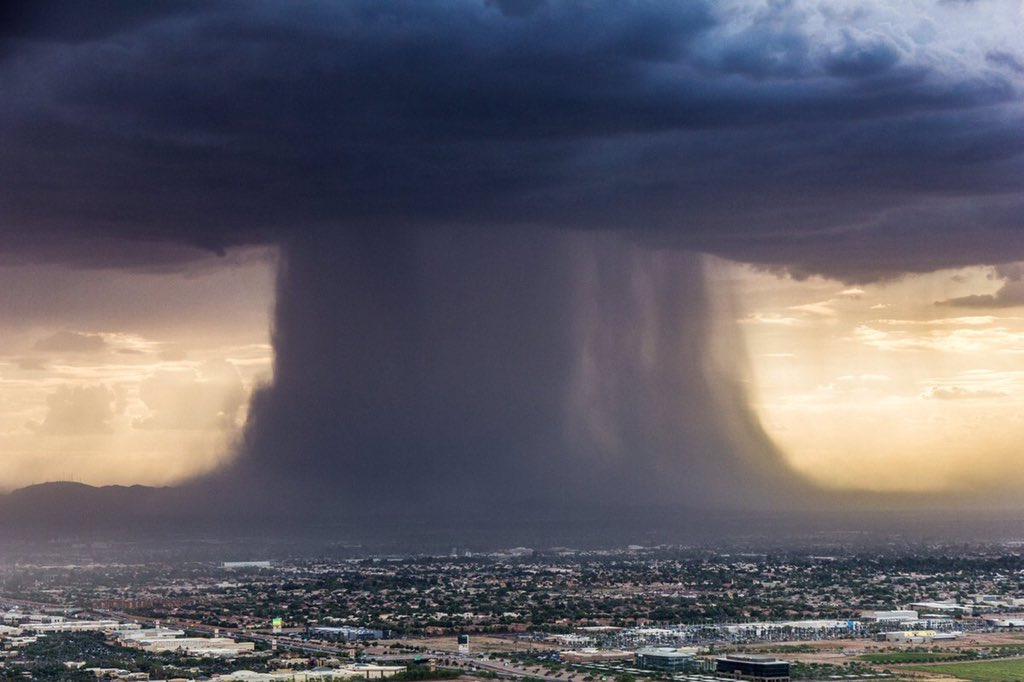
\includegraphics[width=0.8\textwidth]{downburst.jpg}
      \caption{Downburst storm force Phoenix-Arizona.}
		\label{fig:Downburst-force}
	\end{minipage}
\end{figure}

\end{frame}
%%%%%%%%%%%%%%%%%%%%%%%%%%%%%%%%%%%%%%%FRAME%%%%%%%%%%%%%%%%%%%%%%%%%%%%%%%%%%%%%%%%%
\begin{frame}{Numerical results}{Simplified transmission line}
\begin{itemize}
 \item In Uruguay several downburst winds  affects structures and buildings integrity \footnote{https://www.youtube.com/watch?v=-hT5Ak42hww}
 \item Transversal and vertical displacementes are plotted in (2$^{nd}$) stage:
\end{itemize}

\begin{figure}[H]
  \centering
    \includegraphics[width=0.9\textwidth]{SimpifyedLineDisps.JPG}
    \label{fig:LineDisps}
 \end{figure}

\end{frame}
%%%%%%%%%%%%%%%%%%%%%%%%%%%%%%%%%%%%%%% SUB SECTION %%%%%%%%%%%%%%%%%%%%%%%%%%%%%%%%%%%%%%%%%

%\subsection{High voltage Tower}
%%%%%%%%%%%%%%%%%%%%%%%%%%%%%%%%%%%%%%%FRAME%%%%%%%%%%%%%%%%%%%%%%%%%%%%%%%%%%%%%%%%%
%\begin{frame}{Numerical results}{High voltage tower}
%Trabajo colaborativo con Mgs.Ing. Agustín Téliz en ONSAS.
%\pause
%\begin{itemize}
%    \item Truss elements considering geometrical non-linearity.
%    \item Same wind profile illustrated in \ref{{fig:DownburstForce}}
%\end{itemize}


%\begin{figure}[!ht]
%	\begin{minipage}[b]{0.45\linewidth}
%		\centering
%    \includegraphics[width=0.8\textwidth]{SigmaGeneral.png}
 %     \caption{Axial tension superimposed to the tower.}
%		\label{fig:Downburst-force}
%	\end{minipage}
%	\hspace{0.3cm}
%	\begin{minipage}[b]{0.45\linewidth}
%		\centering
   % \includegraphics[width=0.8\textwidth]{DispGneral.png}
  %    \caption{Map of displacementes superimposed to the tower }
%		\label{fig:Downburst-force}
%	\end{minipage}
%\end{figure}

%\end{frame}
%%%%%%%%%%%%%%%%%%%%%%%%%%%%%%%%%%%%%%%FRAME%%%%%%%%%%%%%%%%%%%%%%%%%%%%%%%%%%%%%%%%%

%\begin{frame}{Numerical results}{High voltage tower}
%\begin{itemize}
%    \item Animación del movimiento:
%\end{itemize}


%\end{frame}

%%%%%%%%%%%%%%%%%%%%%%%%%%%%%%%%%%%%%%%FRAME%%%%%%%%%%%%%%%%%%%%%%%%%%%%%%%%%%%%%%%%%

%\begin{frame}{Numerical results}{High voltage tower}
%Safety factor of the structure considering bucking and yield:

%\begin{figure}[H]
 % \centering
   % \includegraphics[width=0.6\textwidth]{WhatsApp Image 2020-08-17 at 20.53.49.jpeg}
%\caption{Safety factor of the hole tower}
 %\end{figure}
%\end{frame}




%%%%%%%%%%%%%%%%%%%%%%%%%%%%%%%%%%%%%%%%     SECTION  %%%%%%%%%%%%%%%%%%%%%%%%%%%%%%%%%%%%%%%%%
\section[Conclusion ]{Conclusions}
\begin{frame}{Conclusions }
\begin{itemize}
 \item A consistent, robust and effective corrotational model was implemented and validated being capable to capture and reproduce large amplitude displacements with a reduced number of elements.
\pause 
 \item This formulation was specifically applied to high voltage transmission lines loaded by wind profiles extracted from recent articles on the subject \cite{Stengel2017a}.
 \pause
 \item The system's responses denotes the excessive sway angle of the conductor, related to this type of loads, the codes developed can be used as a complementary analysis tool for the design of power transmission systems. 
 \pause
 \item Connecting Figure 9 and 10, the identical shape of both profiles can be observed, fulfilling the expectations related to transfer function analysis. 
  
\end{itemize}
\end{frame}
%%%%%%%%%%%%%%%%%%%%%%%%%%%%%%%%%%%%%%%%FRAME%%%%%%%%%%%%%%%%%%%%%%%%%%%%%%%%%%%%%%%%
%%%%%%%%%%%%%%%%%%%%%%%%%%%%%%%%%%%%%%%FRAME %%%%%%%%%%%%%%%%%%%%%%%%%%%%%%%%%%%%%%%%%
\begin{frame}{Questions}

  \begin{block}{¿?}
 			  Doubts? mvanzulli@fing.edu.uy 
 		\end{block}
        
          \begin{block}{Acknowledgment}
 			   This project was financed by the "Compión académica de Postrgrado" of "Universidad de la República" and the "Agenica Nacional de Investigación".
 		\end{block}
\end{frame}


%
\section[Conclusion ]{Future works}
\begin{frame}{Future works }
\begin{itemize}
 \item Verify the non internal slip as published in Foti and Martinelli \cite{foti2018finite}. This hysteresis behaviour depends on the normal forces within the cable, this is essential to ensure the correct modelling of the conductor as a circular solid.
\pause 
\item Implement a model coupled with the tower, where the displacements of the attachment point and the resonance frequencies of the tower are not neglected.
 \pause
\item Finally, it is worth highlighting the potential of this work to develop an integrated solver between the ONSAS-CAFFA software presented in Usera \cite{usera2008parallel}. \cite{usera2008parallel}
 
  
\end{itemize}
\end{frame}


%%%%%%%%%%%%%%%%%%%%%%%%%%%%%%%%%%%%%%%%FRAME%%%%%%%%%%%%%%%%%%%%%%%%%%%%%%%%%%%%%%%%%
\begin{frame}[allowframebreaks]
        \frametitle{Main references}
        \bibliographystyle{abbrv}
        \bibliography{References.bib}
\end{frame}

%%%%%%%%%%%%%%%%%%%%%%%%%%%%%%%%%%%%%%%%FRAME%%%%%%%%%%%%%%%%%%%%%%%%%%%%%%%%%%%%%%%%%
\end{document}
